Опишем задачу более подробно, разделив её на подзадачи:
\begin{enumerate}
\item определить места хранения файлов с личной перепиской пользователя;
\item определить формат файлов переписки;
\item разбор найденных файлов;
\item автоматизировать процесс поиска файлов;
\item производить сохранение полученных информации формат XML.
\end{enumerate}

\subsubsection{Определение местоположения логов переписки мессенджера Skype}

По умолчанию файлы располагаются в директориях, для разных операционных систем возможны незначительные изменения (таблица \ref{tab:skype}). 

\begin{table}[h!]
\caption{Директории хранения логов Skype}
\label{tab:skype}
\begin{tabularx}{\linewidth}{|l|X|}
\hline
Windows Vista/7/8 & C:\textbackslash  Users\textbackslash  username\textbackslash\\ &  AppData\textbackslash  Roaming\textbackslash  Skype\\
\hline
Windows XP & C:\textbackslash  Documents and Settings\textbackslash  username\textbackslash\\ &  Application Data\textbackslash  Skype\\
\hline
Linux(Ubuntu) & /home/username/.Skype\\
\hline
\end{tabularx}
\end{table}

Основная интересующая нас информация находится в main.db \cite{skypechat}. Алгоритм поиска логов представлен на рисунке \ref{pic:list_of_logs}.

%Здесь блок схема алгоритма простого поиска.
\begin{figure}[h]
\center{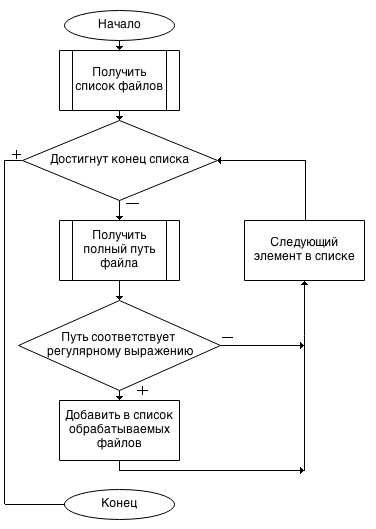
\includegraphics[width=0.6\linewidth]{list_of_logs}}
\caption{Блок-схема алгоритма поиска логов}
\label{pic:list_of_logs}
\end{figure}

\subsubsection{Определение местоположения логов переписки мессенджера Pidgin}

Определение месторасположения файлов переписки происходит следующим образом: для примонтированного образа запускается модуль, который сужает область поиска, сканируя только нужные директории образа. 

По умолчанию файлы располагаются в директориях, для разных операционных систем возможны незначительные изменения (таблица \ref{tab:pidgin}). 

\begin{table}[h!]
\caption{Директории хранения логов pidgin}
\label{tab:pidgin}
\begin{tabularx}{\linewidth}{|l|X|}
\hline
Windows Vista/7/8 & C:\textbackslash Users\textbackslash username\textbackslash  AppData\textbackslash \tabularnewline &  Roaming\textbackslash .purple\textbackslash  logs \tabularnewline 
\hline 
Windows XP & C:\textbackslash  Documents and Settings\textbackslash  username\textbackslash \tabularnewline & Application Data\textbackslash .purple\tabularnewline
\hline 
Windows 98/ME 	& C:\textbackslash Windows\textbackslash Profiles\textbackslash username\textbackslash.purple \tabularnewline
\hline 
Linux(Ubuntu) &	/home/username/.purple/logs \tabularnewline 
\hline
\end{tabularx}
\end{table}

Основная интересующая нас информация хранится в файлах с маской имени \ttfamily YEAR-MONTH-DATE.TIME.html\normalfont (например \ttfamily 2013-03-02.004915+0700NOVT.htm\normalfont).

\subsubsection{Формат хранения переписки мессенджера Skype}

Приложение «skype» хранит переписку на локальных машинах пользователей или же возможна синхронизация с машин других пользователей \cite{skypechat}. Формат хранения: реляционная база данных основная на СУБД SQLite.
Но база данных «main.db» не является единственным местом хранения информации, Skype сохраняет сведения о работе программы во временных файлах (chatsync). Эти файлы имеют расширение «.dat» и цифробуквенные имена (например «0172b0a519e2c584»)\cite{cfl}.

\subsubsection{Формат хранения переписки мессенджера Pidgin}
Приложение «pidgin» поддерживает перечисленные ниже протоколы: \cite{ofpidgin}

\begin{itemize}
\item''AIM''
\item''Bonjour''
\item''Gadu-Gadu
\item''Google Talk''
\item''Groupwise''
\item''ICQ''
\item''IRC''
\item''MSN''
\item''MXit''
\item''MySpaceIM''
\item''SILC''
\item''SIMPLE''
\item''Sametime''
\item''XMPP''
\item''Yahoo!''
\item''Zephyr''
\end{itemize}

Соответственно, все подлюченные аккаунты всех вышеперечисленных протоколов хранятся как лог файлы на локальной машине пользователя в формате HTML и TXT. По умолчанию лог файлы хранятся в .HTML файле. Настройки программы, пользователя и подключенных аккаунтов хранятся в XML.

Примечание: Кроме account.xml - он хранит нешифрованные пароли для всех подключенных чатов \cite{ofpidgin}.

\subsubsection{Алгоритм работы модуля Skype}

Структура рассматриваемого файла.

main.db  содержит 18 таблиц. и ещё немного статистики.

\begin{itemize}
\item''DbMeta''   
\item''Contacts''   
\item''LegacyMessages''
\item''Calls''     
\item''Accounts''   
\item''Transfers''   
\item''Voicemails''   
\item''Chats''      
\item''Messages''   
\item''ContactGroups''  
\item''Videos''   
\item''SMSes''
\item''CallMembers''   
\item''ChatMembers''   
\item''Alerts''
\item''Conversations''     
\item''Participants''   
\item''VideoMessages''
\end{itemize}

Таблицы которые были рассмотрены, на данный момент:    
\begin{enumerate}
\item Contacts
\item Messages
\item Chats
\item Calls
\item CallMembers
\item Conversations
\end{enumerate}

В таблице Contacts находятся все контакты, причем даже те, что были удалены, и уже не показываются в клиенте.

\ttfamily
\noindent select skypename, fullname, languages, country, city from contacts
\normalfont

В таблицах Calls и CallMembers содержатся, соответственно, история звонков и их участников.

\ttfamily
\noindent select calls.id as ''ID разговора'', coalesce(contacts.displayname, accounts.fullname) as ''Инициатор'', strftime('\%d.\%m.\%Y \%H:\%M:\%S',calls.begin\_timestamp, 'unixepoch', 'localtime') as ''Дата начала'', time(calls.duration, 'unixepoch') as ''Длительность'', callmembers.dispname as ''Подключенный участник'', strftime('\%d.\%m.\%Y \%H:\%M:\%S',callmembers.start\_timestamp, 'unixepoch', 'localtime') as ''Дата подключения'', time(callmembers.call\_duration, 'unixepoch') as ''Длительность подключения'' from calls inner join callmembers on calls.id = callmembers.call\_db\_id left  join contacts on calls.host\_identity = contacts.skypename left  join accounts on calls.host\_identity = accounts.skypename
\normalfont

И, наконец, в таблицах Conversations и Messages содержатся данные переписки и сами сообщения.

\ttfamily
\noindent select conversations.id as ''ID переписки'', conversations.displayname as ''Участники переписки'', 
       messages.from\_dispname as ''Автор сообщения'',
       strftime('\%d.\%m.\%Y \%H:\%M:\%S',messages.timestamp, 'unixepoch', 'localtime') as ''Время сообщения'', 
       messages.body\_xml as ''Текст сообщения''
  from conversations
       inner join messages on conversations.id = messages.convo\_id
order by messages.timestamp
\normalfont

Для доступа ко всему содержимому базы достаточно иметь доступ к самому файлу — содержимое базы никак не шифруется и не защищается, так что любой человек, который сможет получить доступ к вашему профилю Windows, сможет найти список контактов, просмотреть историю звонков и прочитать всю переписку. 

\subsubsection{Алгоритм работы модуля Pidgin}

Структура рассматриваемого файла. 

У каждого лог файла есть заголовок находящийся между тегов title. В котором записан ID\_Chat, дата начала переписки, логин пользователя и используемый протокол.

Затем идет ''тело'' в котором описывается обмен сообщениями в формате, время, автор сообщения и сообщение.

Пример ''Заголовка'' \ttfamily <head><meta http-equiv = ''content-type'' content= ''text/html; charset=UTF-8''> <title> Conversation with 0dpkhcz6clufs2kozj82uqif30@public.talk.google.com at Чт. 24 окт. 2013 23:40:21 on user.fox@gmail.com/ (jabber)</title></head>\normalfont

Пример ''Тела'' \ttfamily <font color=''\#16569E''> <font size=''2''> (23:44:52) </font> <b>user.fox@gmail.com/95C9F047: </b></font> Hello) <br/>\normalfont

Точно так же из полученного списка найденные файлы поочередно открываются для чтения. Разбор открытого файла решено осуществлять при помощи регулярных выражений, описанных в класс QRegExp.

%Здесь блок схема алгоритма парсинга файлов пиджина
Парсинг логов pidgin представлен на рисунке \ref{pic:Pars_pidgin_log}.

\begin{figure}[h]
\center{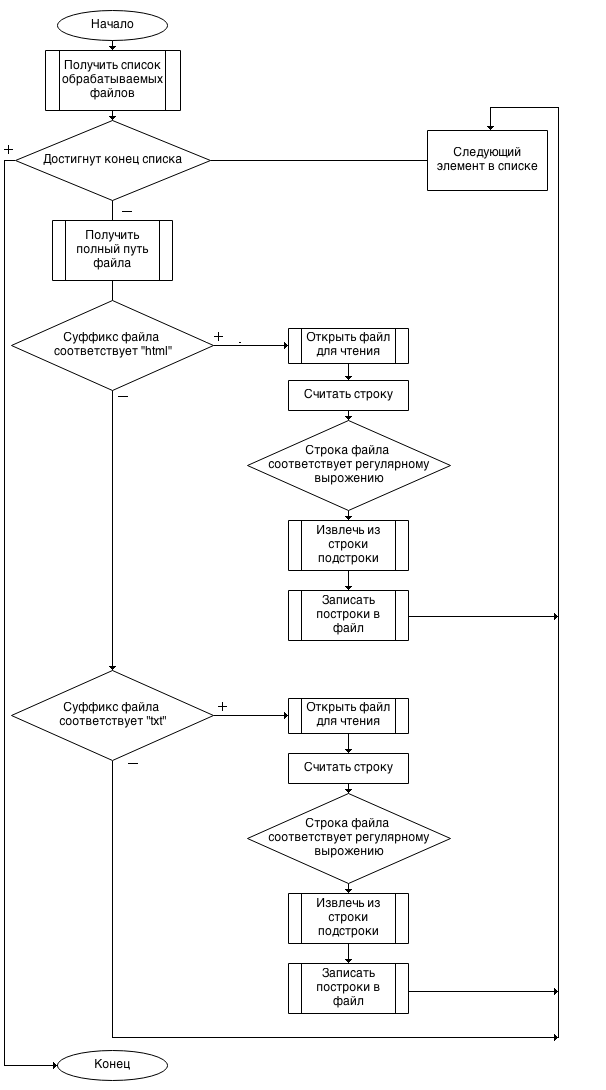
\includegraphics[width=0.5\linewidth]{Pars_pidgin_log}}
\caption{Блок-схема алгоритма парсинга логов}
\label{pic:Pars_pidgin_log}
\end{figure}

\subsubsection{Структура логов Skype, сохранённых в XML}

Все документы XML начинаются с пролога (prolog). Пролог сообщает, что документ написан на XML, а также указывает, какая версия XML при этом использовалась.  

Следующий элемент Messages с атрибутом Messenger, ему присваивается имя рассматриваемого приложения.

Для каждого файла БД, находящейся в обрабатываемом списке, создается элемент info account содержащий атрибуты skypeName, fullName, emails, ipcountry которым присваивается, соответственно: логин пользователя Skype, его полное имя, email (не шифрованный), геолокация ip-адреса.  

Далее следует элемент contact содержащий атрибуты skypeName, fullName, languages, country, city.

Пример выходного файла в формате XML представлен на рисунке \ref{pic:log_skype}.
  
\begin{figure}[h]
\center{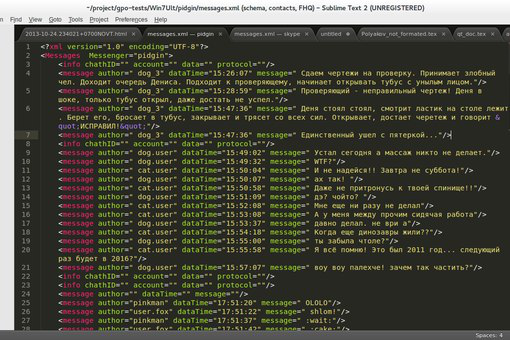
\includegraphics[width=0.9\linewidth]{log_skype}}
\caption{логи Skype в формате XML}
\label{pic:log_skype}
\end{figure}

\subsubsection{Структура логов Pidgin, сохранённых в XML}

Все документы XML начинаются с пролога (prolog). Пролог сообщает, что документ написан на XML, а также указывает, какая версия XML при этом использовалась.  

Следующий элемент Messages с атрибутом Messenger, которому присваивается имя рассматриваемого приложения.

Далее следует элемент INFO содержащий атрибуты chathID, account, data, protocol которым присваивается, соответственно: идентификатор чата, полная дата в формате День.Число Месяц. Год Час:Мин:Сек, аккаунт с которого происходил обмен сообщениями и протокол используемый для передачи сообщений. 

Последний элемент -- MESSAGE, содержащий атрибуты author, dataTime, message.

Пример выходного файла в формате XML представлен на рисунке \ref{pic:log_pidgin}.

\begin{figure}[h]
\center{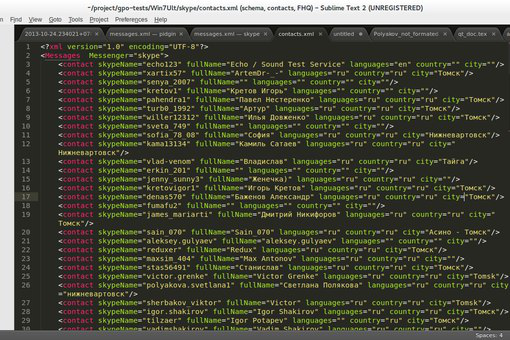
\includegraphics[width=0.9\linewidth]{log_pidgin}}
\caption{логи Pidgin в формате XML}
\label{pic:log_pidgin}
\end{figure}

На текущий момент полностью реализован импорт контактной книги из приложения Skype, импорт звонков и переписки находится в режиме разработки.
